\documentclass[tikz,crop]{standalone}

\usepackage[T1]{fontenc}
\usepackage{multirow, makecell}
\usepackage[tt=false,type1=true]{libertine}
%%% \usepackage[varqu]{zi4}
%%% \usepackage{newtxmath}
\usepackage{listings}
\usepackage[dvipsnames]{xcolor}
\usepackage{tikz}
%%% \usepackage{bbding}
\usetikzlibrary{arrows,backgrounds,external,fit,positioning,shadows,shapes,shapes.arrows,shapes.multipart}
% \tikzexternalize

% COLORS: https://colorkit.co/palette/c7522a-e5c185-fbf2c4-74a892-008585/
\definecolor{palet1}{HTML}{c7522a}
\definecolor{palet2}{HTML}{e5c185}
\definecolor{palet3}{HTML}{fbf2c4}
\definecolor{palet4}{HTML}{74a892}
\definecolor{palet5}{HTML}{008585}
\colorlet{ctile}{palet1}
\colorlet{cinterchange}{palet2}
\colorlet{cfuse}{palet4}
\colorlet{cshift}{palet3}
\colorlet{csplit}{palet5}
\colorlet{cscale}{white}

\lstset{
    % backgroundcolor=\color{backcolour},
    % stringstyle=\color{codepurple},
    % commentstyle=\color{codegreen},
    keywordstyle=\bfseries\color{magenta},
    numberstyle=\tiny\color{codegray},
    basicstyle=\ttfamily\tiny,
    % captionpos=b,
    escapeinside={/@}{@/},
    % breakatwhitespace=false,
    % breaklines=true,
    % keepspaces=true,
    % numbers=left,
    % numbersep=5pt,
    % showspaces=false,
    % showstringspaces=false,
    % showtabs=false,
    % tabsize=2
}

% \colorlet{ml-model-bg}{CornflowerBlue!10}

\begin{document}
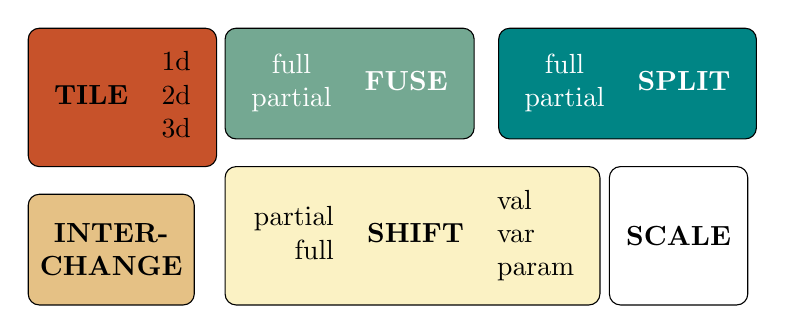
\begin{tikzpicture}[
  t/.style={draw, rounded corners, anchor=north west}
  ]

  % TILE
  \node[t,fill=ctile,minimum width=6em, minimum height=5em] (tile) at (0,0) {
    \begin{tabular}{cl}
      \multirow{3}*{\textbf{TILE}} & 1d \\
      & 2d \\
      & 3d
    \end{tabular}
  };

  % INTERCHANGE
  \node[t,fill=cinterchange,align=center,minimum width=6em, minimum height=4em] (interchange) at (0, -6em) {
    \textbf{INTER-} \\ \textbf{CHANGE}
  };

  % FUSE
  \node[t,fill=cfuse, text=white, minimum width=9em, minimum height=4em] (fuse) at (2.5,0) {
    \begin{tabular}{cl}
      full & \multirow{2}*{\textbf{FUSE}} \\
      partial &
    \end{tabular}
  };

  % SPLIT
  \node[t,fill=csplit,text=white, minimum width=9em, minimum height=4em] (split) at (17em, 0) {
    \begin{tabular}{cl}
      full & \multirow{2}*{\textbf{SPLIT}} \\
      partial &
    \end{tabular}
  };

  % SHIFT
  \node[t,fill=cshift, minimum height=5em] at (2.5, -5em) (shift) {
    \begin{tabular}{rcl}
      \multirow{3}{3em}{\makecell[r]{partial\\full}}& \multirow{3}*{\textbf{SHIFT}} & val \\
      & & var \\
      & & param
    \end{tabular}
  };

  % SCALE
  \node[t,fill=cscale, minimum width=5em, minimum height=5em] (scale) at (21em, -5em) {
    \textbf{SCALE}
  };

\end{tikzpicture}
\end{document}
